\documentclass[main]{subfiles}
\begin{document}
%@@@@@@@@@@@@@@@@@@@@@@@@@@@@@@
% summarizes lecture 2
% author: David Bontrager, Benjamin Ellenberger and Joachim Ott

%Joachim Start
\section{MOSFETs}
Metal-Oxide-Semiconductor Field-Effect Transistor \footnote{Metal-Oxide-Semiconductor [what it's made of] Field Effect Transistor [how it works]}, built using MOS and a p-n junction diode.

\subsection{MIS and MOS structure}

\subsubsection{MIS}  Metal-Insulator-Semiconductor, consists of a conductor and a semiconductor, separated by thin insulation layer.
\subsubsection{MOS}  Metal-Oxide-Silicon, a version of MIS, in which silicon dioxide ($SiO_2$) is used as oxide.

The traditional metal–oxide–semiconductor (MOS) structure is obtained by growing a layer of silicon dioxide ($SiO_2$) on top of a silicon substrate and depositing a layer of metal or polycrystalline silicon (the latter is commonly used). As the silicon dioxide is a dielectric material, its structure is equivalent to a planar capacitor, with one of the electrodes replaced by a semiconductor.

When a voltage is applied across a MOS structure, it modifies the distribution of charges in the semiconductor. If we consider a p-type semiconductor (with $N_A$ the density of acceptors, p the density of holes; p = $N_A$ in neutral bulk), a positive voltage, $V_{gb}$, from gate to body (see figure \ref{fig:MOS_Structure}) creates a depletion layer by forcing the positively charged holes away from the gate-insulator/semiconductor interface, leaving exposed a carrier-free region of immobile, negatively charged acceptor ions.
\begin{figure}[H]
\centering
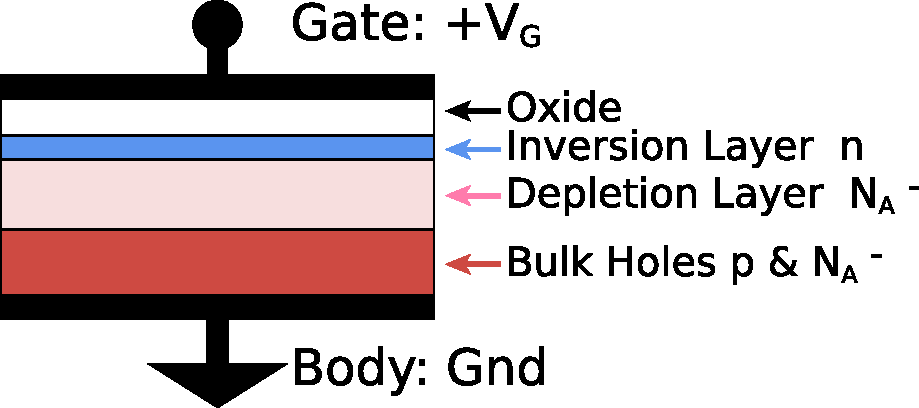
\includegraphics[width=0.6\linewidth]{figs/MOS_Capacitor.pdf}
\caption{Metal–oxide–semiconductor structure on p-type silicon.}
\label{fig:MOS_Structure}
\end{figure}
 If $V_{gb}$ is high enough, a high concentration of negative charge carriers forms in an inversion layer located in a thin layer next to the interface between the semiconductor and the insulator. Unlike the MOSFET, where the inversion layer electrons are supplied rapidly from the source/drain electrodes, in the MOS capacitor they are produced much more slowly by thermal generation through carrier generation and recombination centers in the depletion region. Conventionally, the gate voltage at which the volume density of electrons in the inversion layer is the same as the volume density of holes in the body is called the threshold voltage. When the voltage between transistor gate and source ($V_{gs}$) exceeds the threshold voltage ($V_{th}$), it is known as overdrive voltage.

This structure with p-type body is the basis of the n-type MOSFET, which requires the addition of an n-type source and drain regions \cite{wiki:MOSFET}.

\subsection{MOS Transistor Structure}

\subsubsection{CMOS}  Complementary Metal Oxide Silicon, a MOS process in which both nFET and pFET are fabricated on the same substrate.
\subsubsection{MOSFET} Metal-Oxide-Semiconductor Field-Effect Transistor, built using MOS and a p-n junction diode.

The metal–oxide–semiconductor field-effect transistor (MOSFET, MOS-FET, or MOS FET) is a type of transistor used for amplifying or switching electronic signals.
In neuromorphic engineering, we use the MOSFET in the subthreshold domain because the current here is exponentially dependent on the control voltages of the MOSFET just as the ionic conductances of a neuron are exponentially dependent on its membrane potential. Furthermore when MOSFETs are operated in the subthreshold domain, they draw small currents so power consumption is reduced.

\begin{figure}[H]
  \centering

  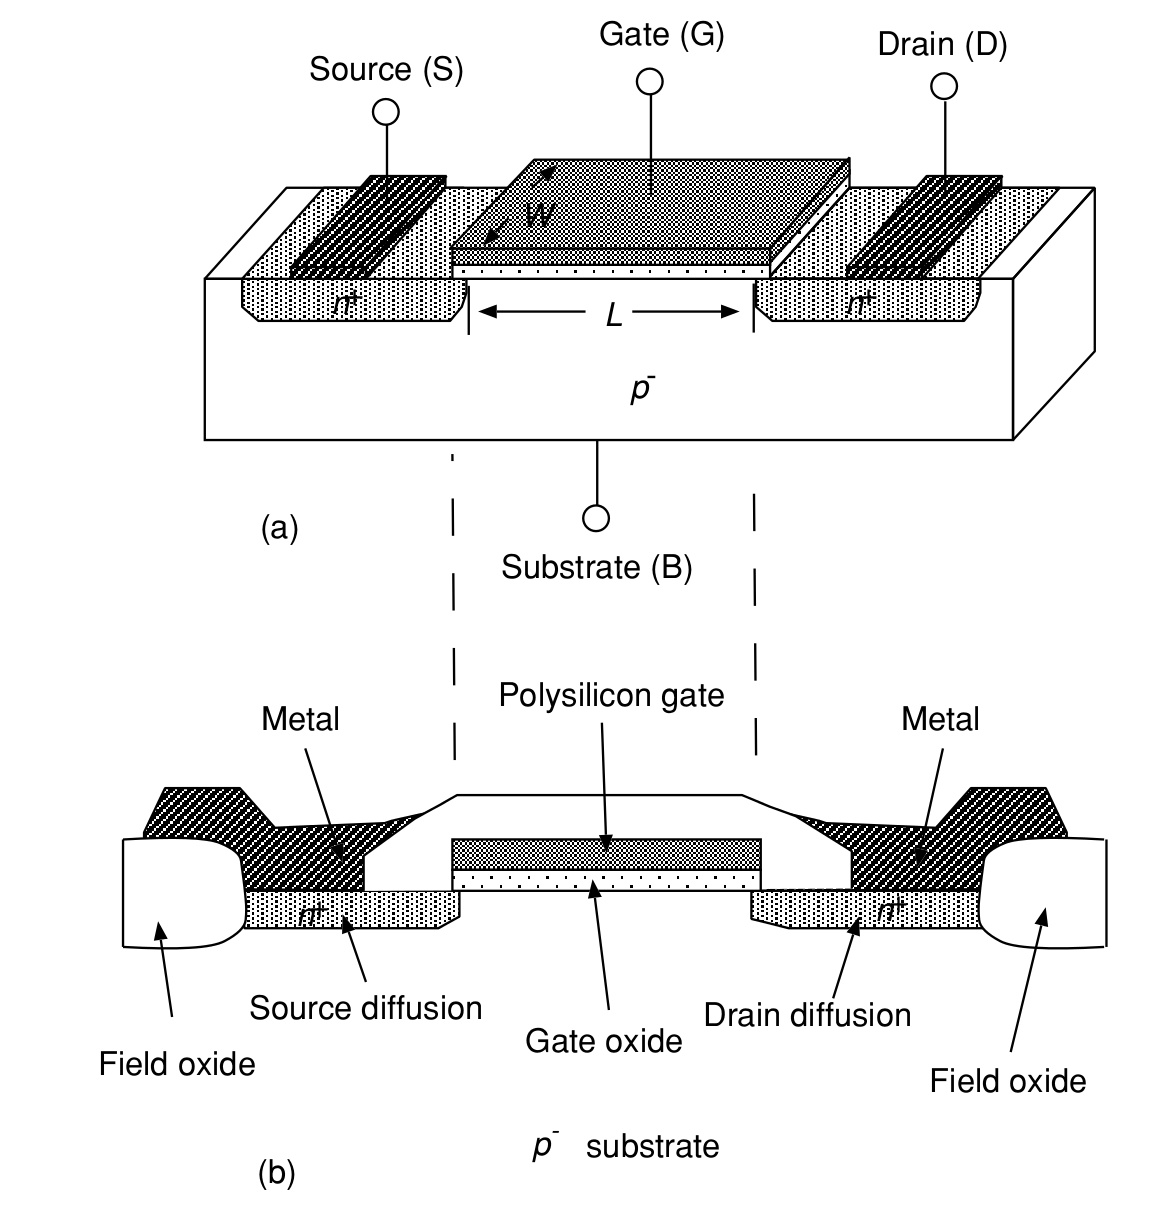
\includegraphics[scale=0.8]{figs/MOSFET_Structure.jpg}
  \caption{Structure of an n-type MOSFET in a p-body. The MOSFET has four terminals; the drain (D), the source (S), the gate (G), and the bulk (B). (a) Pictorial view of the MOSFET. (b) A more realistic picture of a cross-section of a fabricated MOSFET. Note that the gate oxide is much thinner than the field oxide. \cite{book:VLSI}}
  \label{fig:MOSFET_Structure}
\end{figure}\bigskip

\subsection{MOS Transistor Types}
\subsubsection{n-type}
    Because the n+ source and drain regions can supply a lot of electrons to the channel, this device is called an n-channel MOSFET (nFET,n-type MOSFET, NMOS) \cite{book:VLSI}
\subsubsection{p-type}
   In p-channel MOSFET (pFET,p-type MOSFET, PMOS) , the charge in the channel is carried by holes supplied from the source and drain regions.
    
\bigskip\subsection{MOS Transistor in Substrate}
Most CMOS processes use a p-type starting substrate.  The nFETs rest in the common $p^-$ substrate, and the pFETs rest in
n-wells within the substrate as shown in Fig. \ref{fig:MOSFET_Physical_Structure}

\begin{figure}[H]
  \centering
  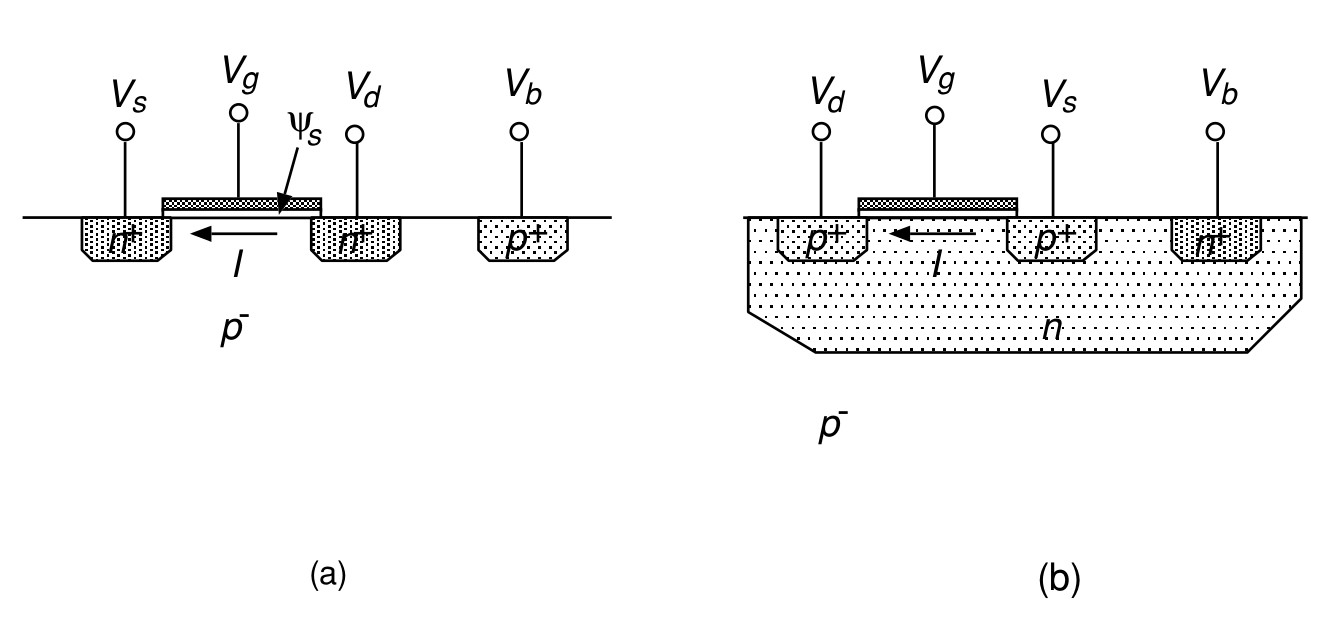
\includegraphics[scale=0.8]{figs/MOSFET_Physical_structure.jpg}
  \caption{Physical structure of (a) an nFET and (b) a pFET in a common $p^-$ substrate. The pFET rests in a n-well within the substrate. \cite{book:VLSI}}
  \label{fig:MOSFET_Physical_Structure}
\end{figure}

\subsection{Transistor biasing}
For a transistor to work properly, we need certain bias conditions.
These bias conditions guarantee that there will only be a small reverse leakage current at these junctions and that most of the transistor’s current will flow in the channel.
\subsubsection{nFET biasing}
To ensure only a small leakage current between the $n^+$ regions to the p-substrate, the junctions have to be reverse biased.
To do this, the drain voltage $V_d$ and the source voltage $V_s$ of the nFET should be greater than or equal to the bulk voltage $V_b$:
\[V_{sb}=V_s-V_b \geq 0\]
\[V_{db}=V_d-V_b \geq 0\]


The $n^+$ region biased at the higher voltage is called the drain, and the other $n^+$ region is called the source. Because electrons are negatively charged, the direction of positive current flow $I$ is from drain to source, even though the carriers flow from source to drain. The bulk of the nFET is tied to the lowest voltage ( $V_{ss}$ ). \cite{book:VLSI}

\subsubsection{pFET biasing}
In pFET , the $p^+$ regions should be biased negative relative to the bulk to reverse-bias the pn junctions.
\[V_{sb} \leq 0\]
\[V_{db} \leq 0\]
The n-type bulk (or n-well) of the pFET should be biased higher (usually $V_{dd}$.  In a $p^-$ substrate, where the pFET rests in an n-well, the well is connected to $V_{dd}$, and the substrate to $V_{ss}$.) For a pFET, the $p^+$ region which is biased at the higher voltage is called the source and the other $p^+$ region is called the drain.

\begin{figure}[H]
\centering
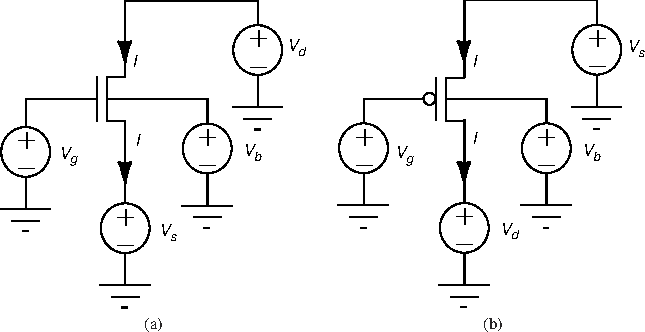
\includegraphics[width=0.8\linewidth]{figs/nFET-pFET-operation.pdf}
\caption{Biased MOSFETs showing the direction of conventional current flow. (a) For proper nFET operation, we should ensure that $V_g \geq V_b, V_s \geq V_b $ and $V_d \geq V_b$. If $V_d \geq V_s$, the channel current $I$ is positive, flowing from drain to source as shown. If $V_d \leq V_s$, then $I$ is negative and flows in the opposite direction. (b) For proper pFET operation, we should ensure that $V_g \leq V_b, V_s \leq V_b $ and $V_d \leq V_b$. If $V_d \leq V_s$, the channel current $I$ is positive, flowing from drain to source as shown. If $V_d \geq V_s$, then $I$ is negative and flows in the opposite direction.}
\end{figure}


\subsection{MOS Transistor Channel}
The region underneath the gate and between the source and drain regions is called the channel. The channel has a width W, and a length L. The channel is insulated from the gate above by a layer of silicon dioxide. The gate is made of heavily doped (low resistivity) polycrystalline silicon.
\cite{book:VLSI}

\subsection{MIS Operation Domains}
In a typical MIS structure, the insulator layer is sufficiently thick that it cannot be crossed by charge carriers under normal operating conditions and sufficiently thin that the charge on the conductor can influence the charge distribution in the semiconductor via the electrostatic potential it induces. A positive
charge on the conductor attracts mobile electrons from the semiconductor to
the semiconductor-insulator interface and repels mobile holes away from the
interface. Conversely, a negative charge on the conductor attracts holes and
repels electrons.\\
\textbf{Important: }Relevant here is the type of substrate (p-type or n-type) the channel is made of, which is p-type in nFET and n-type in pFET!
\begin{figure}[H]
  \centering
  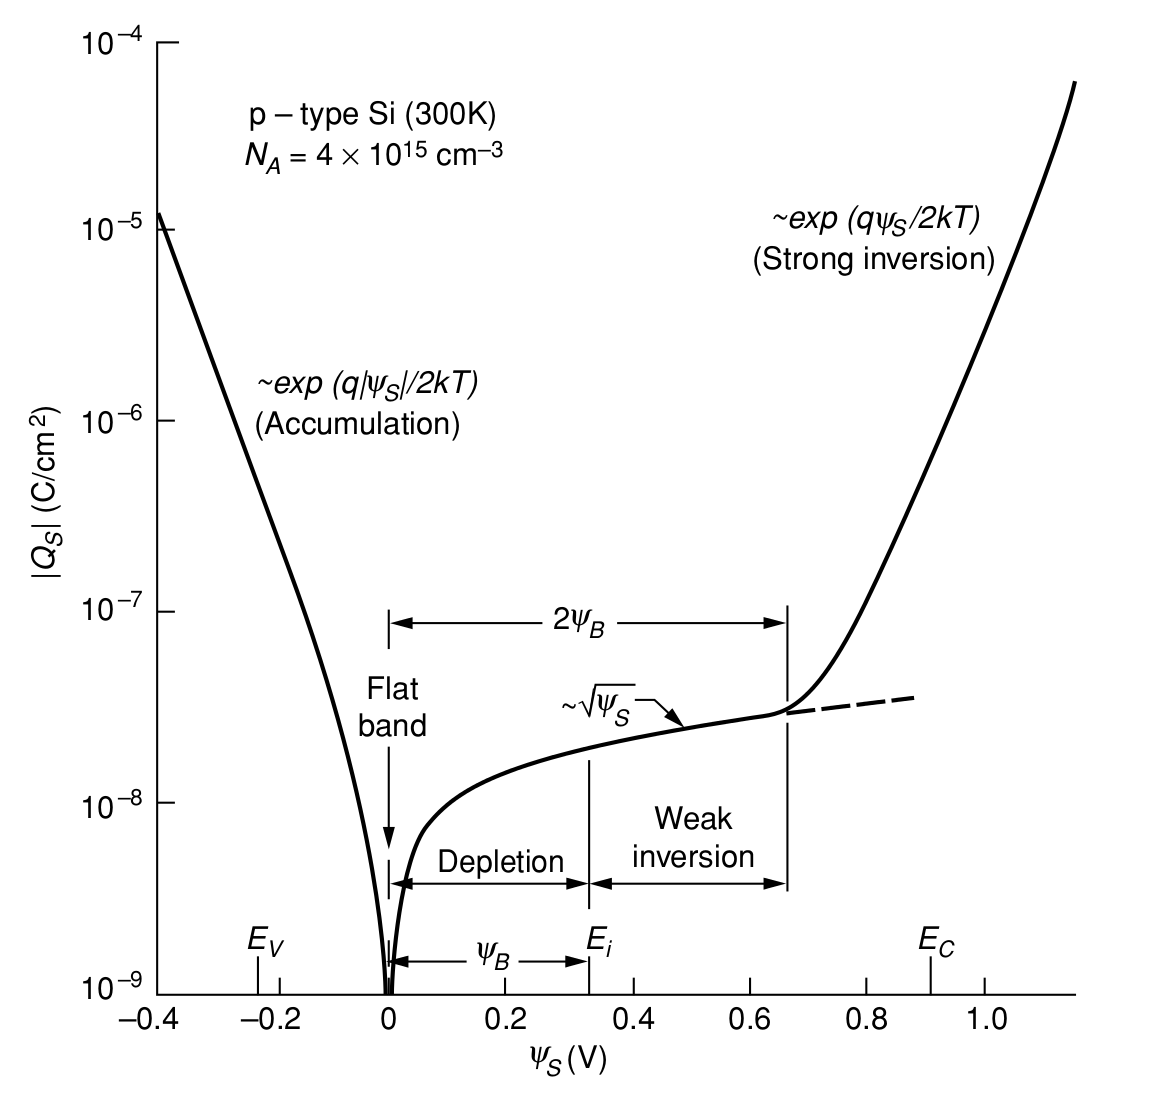
\includegraphics[scale=1]{figs/operation_domains.png}
  \caption{Dependence of the area charge $Q_s$ on the surface potential for p-type silicon with acceptor density $N_A = 4 \times \unit[10^{15}]{cm^{-3}}$ at room temperature. The same effects are observed in n-type semiconductors, if the sign of the charge on the conductor is reversed \cite{book:VLSI}.}
  \label{fig:coperation_domains}
\end{figure}

\begin{figure}[H]
\centering
  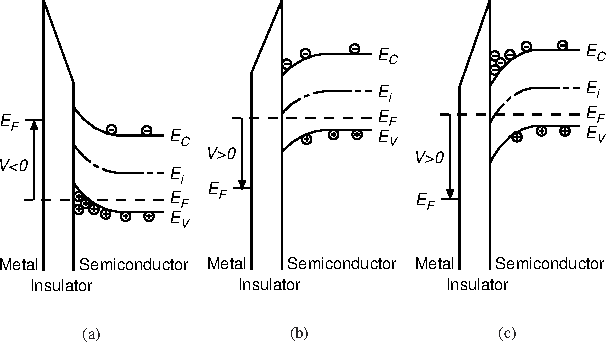
\includegraphics[scale=1]{figs/operation_domains2.pdf}
  \caption{Energy-band diagrams of an ideal MIS diode with applied bias for a p-type semiconductor in (a) accumulation, (b) depletion, and (c) inversion \cite{book:VLSI}.}
\end{figure}

\subsubsection{Accumulated Transistor Channel}
Accumulation happens when a charge on the gate attracts a lot of majority carriers on the surface of the semiconductor (the bulk/substrate) underneath it.\\
For a p-substrate channel (default), as shown in figure \ref{fig:channel_accumulated}, a negative voltage on the gate means mobile electrons on the gate. These electrons (negatively charged) attract positive charges on the semiconductor surface underneath it, leading to accumulation of them. Since positive charges (holes) are the majority carrier in p-substrate, we call this situation accumulation.\\\\
In a n-substrate channel, positive charge on the gate leads to accumulation of electrons (majority carriers in n-substrate) on the channel surface.
\begin{figure}[H]
  \centering
  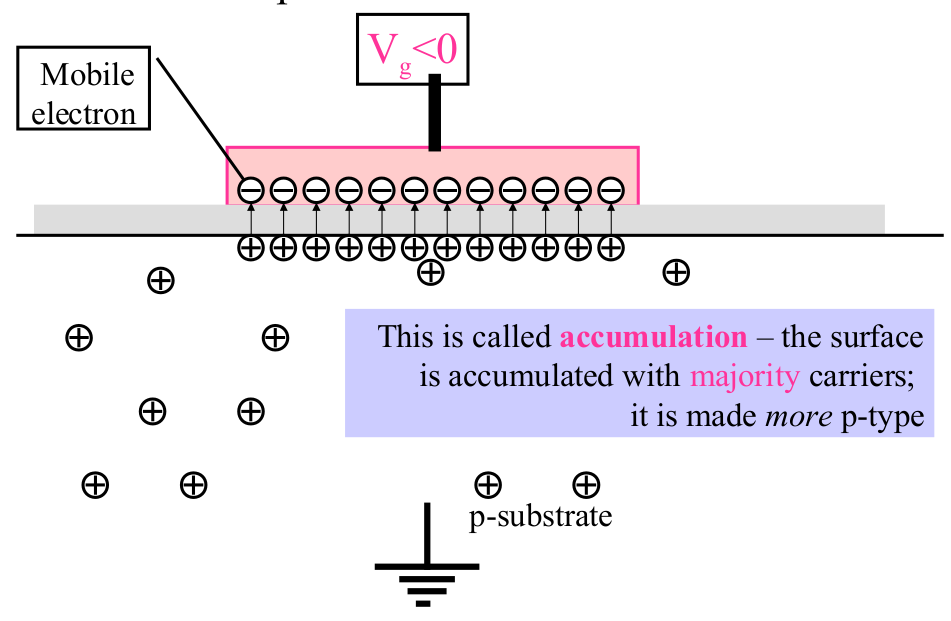
\includegraphics[scale=1]{figs/channel_accumulation.png}
  \caption{Accumulated Transistor Channel \cite{lec2}}
  \label{fig:channel_accumulated}
\end{figure}


\subsubsection{Flat-Band Transistor Channel}
In an ideal MIS diode, with no bias applied, the work function of the metal and the semiconductor are the same.  The Fermi levels line up and the energy bands in the semiconductor are flat. $\rightarrow$ Flat-Band Condition \cite{book:VLSI}\\
With $V_g=V_{fb}=0$, the majority carrier density is constant and equal to the dopant density.
\begin{figure}[H]
  \centering
  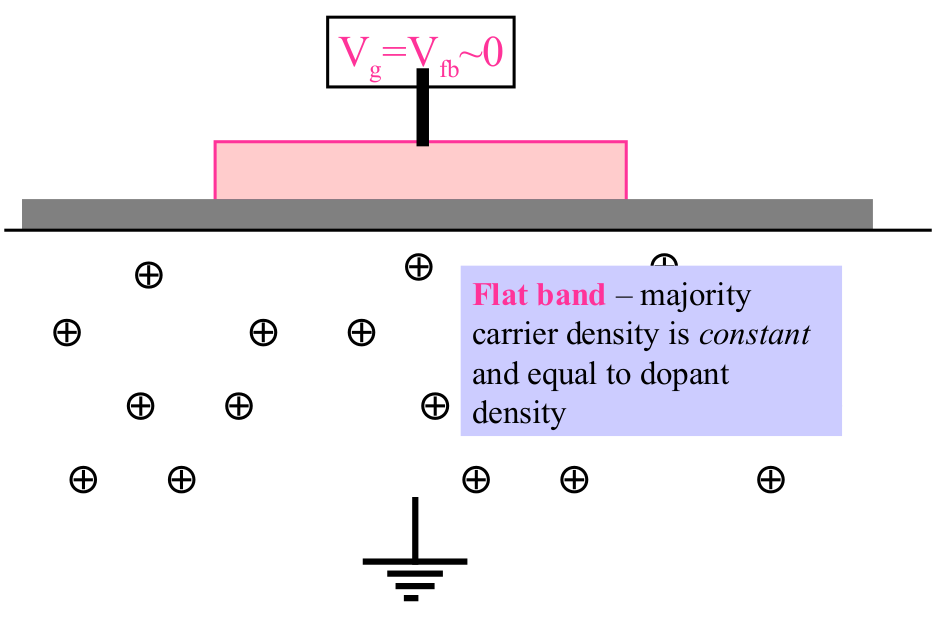
\includegraphics[scale=1]{figs/channel_flat_band.png}
  \caption{Flat-Band Transistor Channel \cite{lec2}}
  \label{fig:channel_flat_band}
\end{figure}

\subsubsection{Depleted Transistor Channel}

For a p-substrate channel, if we put a positive subthreshold voltage on the gate (positive charges), we repulse positive majority carriers on the semiconductor surface. $\rightarrow$ Depletion of majority carriers.\\
For a n-substrate channel, the same happens if we put a subthreshold negative charge on the gate. $\rightarrow$ Depletion of electrons (majority carrier in n substrate) on the semiconductor surface.

\begin{figure}[H]
  \centering
  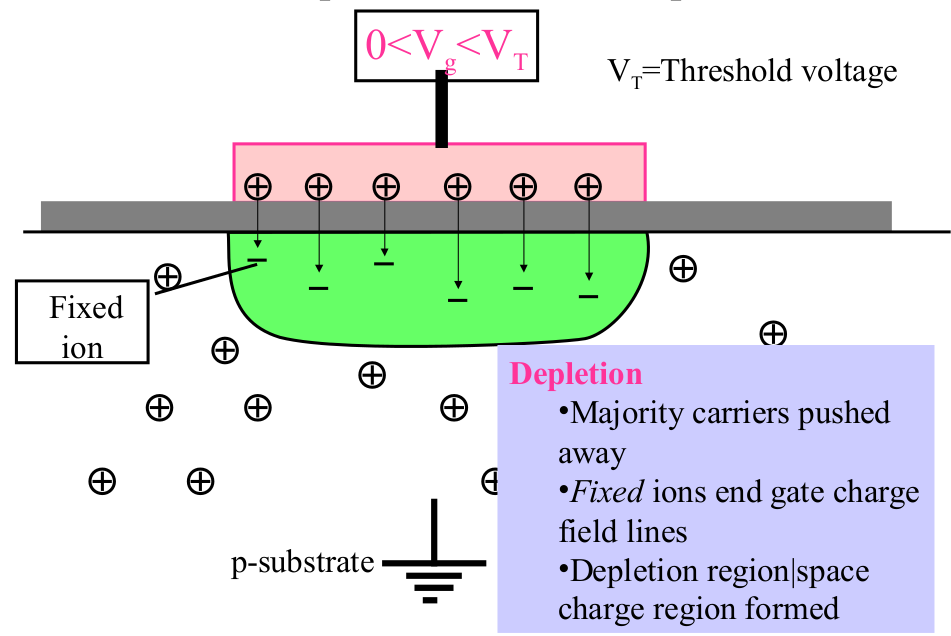
\includegraphics[scale=1]{figs/channel_depletion.png}
  \caption{Depleted Transistor Channel \cite{lec2}}
  \label{fig:channel_depletion}
\end{figure}

\subsubsection{Inverted Transistor Channel}
For a depleted p-substrate channel, if we now further increase the positive charge on the gate, we will reach a point where we start attracting negative minority carriers on the semiconductor surface. The surface becomes inverted. (p-type $\rightarrow$ n-type and vice versa in n substrate)  $\rightarrow$ Inversion
\begin{figure}[H]
  \centering
  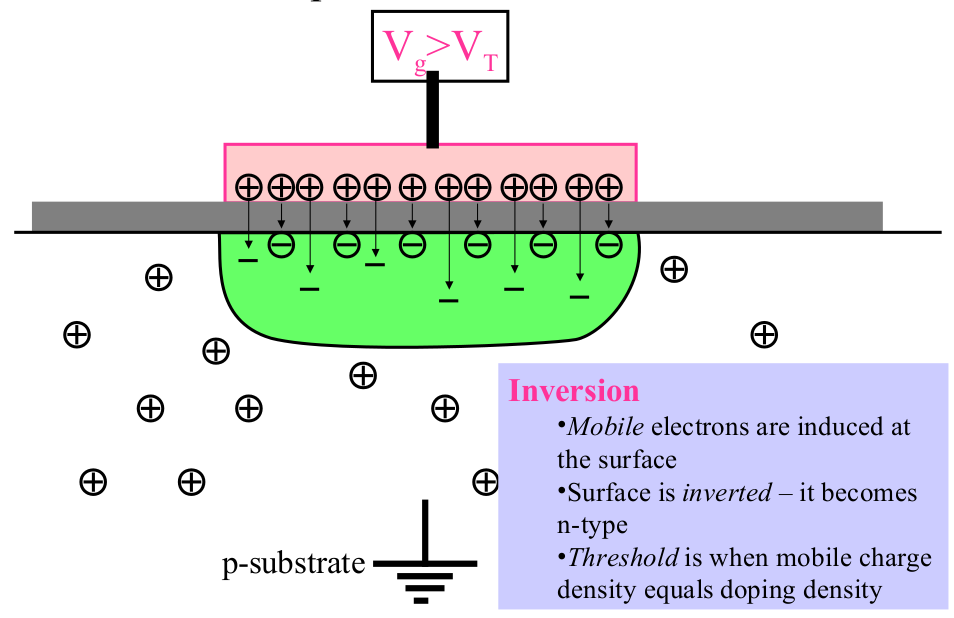
\includegraphics[scale=1]{figs/channel_inversion.png}
  \caption{Inverted Transistor Channel \cite{lec2}}
  \label{fig:channel_inversion}
\end{figure}
%Joachim End
%Ben Start
\subsubsection{Strongly Inverted Transistor Channel}
The minimum voltage that has to be applied to the MIS structure to obtain
strong inversion is called threshold voltage.

\subsection{n- and p-FETs, in an n–well Process}

A MOSFET is a type of transistor that consists of  two p-n junctions, called either native transistors or well transistors depending on the composition of the p-type and n-type substrates. Native transistors sit in the substrate wafer doping type (or in wells of the same type as the substrate). The native transistor contains of two n-doped terminals and the gate. It is called native, because it is directly located in the p substrate. The pn junction is thereby given between the substrate and the n-doped terminals. Native transistors have n-type sources and drains and form an n-type channel in the p-substrate. \\ Well transistors sit in wells of the opposite type as the substrate. The well transistor in the p substrate needs an additional terminal, because its terminals are p-doped. An n-well chip for instance sits in an n-well and the substrate is p-type.  The well has p-type sources and drains and forms a p-channel in the n-well.
\begin{figure}[H]
\centering
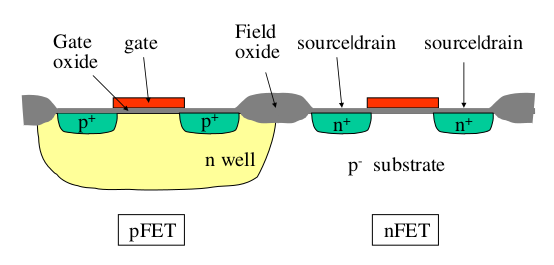
\includegraphics[width=0.6\linewidth]{figs/Field-effect-transistors.png}
\caption{Cross-section of a complementary pair of Field-Effect Transistor (FET)}
\label{field-effect transistor}
\end{figure}

FETs are generally symmetrical and the names of the terminals are defined by how it is connected. In an n-FET, electrons are transported through an electron channel. In a p-FET, electron holes are transported through an electron hole channel. Thus, the source terminal of the transistor is defined as the source of the majority carriers, which are electrons or electron holes respectively.\\

\subsection{MOSFET operation domains}
%David
The operation domain of an nFET is set by the relative values of the four terminals of the transistor.\\
In general, these operation domains (e.g. accumulation, depletion, weak inversion, moderate inversion, or strong inversion) are equivalent to the ones of the MIS structure.\\
We know about the sub- and above threshold regions. Moving between these two regions is a function of $V_g$, specifically the voltage between the gate and the source ($V_{gs} = V_g - V_s$). Both the sub- and the above threshold regions are divided into the triode\footnote{Interesting but irrelevant: ``triode'' comes from the original thought behind the transistor as a 3-terminal diode, thus \emph{tri-}ode vs. \emph{di}-ode. The entire transistor history on Wikipedia is a really interesting read.} and saturation regimes. For both sides of the threshold, we move in and out of saturation by changing $V_{ds}$ – the drain-source voltage.\\ \\
\textsl{This is important: changing \emph{gate-source} voltage from low to high moves us from subthreshold to above threshold for \emph{any} $V_{ds} > 0$. Similarly, changing \emph{drain-source} voltage from low to high moves us from ohmic regime to saturation regime for \emph{any} $V_{gs} > 0$.} \\ \\

We can map the regimes to a MOSFET mode:


\begin{longtable}{ |p{4.5cm}|p{3.5cm}|p{4.5cm}| }
\hline
\textbf{When the MOSFET is in this domain: \newline (depending on $V_{gs}$)} & \textbf{We say the MOSFET operates in:} & \textbf{Which can be further divided into regimes: \newline (depending on $V_{ds}$)} \\ \hline
\endhead
Accumulation & Cutoff & \\ \hline
Depletion & Cutoff & \\ \hline

Weak Inversion & Subthreshold & Triode Mode \par Saturation Mode\\ \hline
 Strong Inversion & Above Threshold & Triode Mode \par Saturation Mode\\ \hline
\end{longtable}

\subsubsection{Subthreshold Region}
Increasing the gate voltage increases the positive charge on the gate. This
charge repels the holes in the substrate and leaves behind negatively-charged
ions, that balance out the gate charge. The MOSFET operates in the sub-
threshold regime when the positive charge on the gate is almost balanced by
the negatively-charged depletion region underneath the gate.
There is also a very thin layer of electrons beneath the gate (the inversion
layer).

\subsubsection{The coupling factor $\kappa$}
Surface voltage $\psi_s$ deserves another mention. We've built a transistor, plugged it in, and biased the gate relative to the bulk\footnote{Really, we care about all voltages \emph{relative to the bulk}, but bulk is almost always at ground so it's an implicit relation}. Because of the positive gate voltage, the depletion region does not only surround the drain and source, but also extends between them. Having this channel of depletion region means that there is a built-in voltage across it\footnote{Not across it as in a \emph{drain-source} voltage, but across it as in perpendicular to the plane of the insulating oxide}. So here we have two voltages in series – one across the insulating oxide, one across the depletion region. Current isn't flowing across either of these gradients, so what does that mean? It means static, accumulated charges are hanging out on either side of the gradients. In other words: they are capacitances. The relationship between the capacitances is described by $\kappa$, which we call the \textsl{capacitive coupling ratio} from gate to channel. It describes how effectively a change in gate voltage can change the surface voltage.
The relationship between the applied potential and the surface potential is given by the coupling factor

\[\pl{\kappa = \frac{C_{ox}}{C_{ox} + C_{dep}} = \frac{\partial\psi_s}{\partial V_g}}\]

which is the incremental capacitive divider ratio as seen from the conductor
side.
%david

\end{document}